\documentclass[border=2pt]{standalone}
\usepackage[T1]{fontenc}
\usepackage[scaled=1.0]{helvet}
\renewcommand{\familydefault}{\sfdefault}
\usepackage{sfmath}
\usepackage{amsmath}
\usepackage{xcolor}
\usepackage{tikz}
\usetikzlibrary{positioning,arrows.meta,calc,fit,backgrounds,shapes.geometric}
% palette (light fills, dark strokes: prints well in colour and greyscale)
\definecolor{ink}{HTML}{1F2933}
\definecolor{muted}{HTML}{52606D}
\definecolor{dataS}{HTML}{B7791F}\definecolor{dataF}{HTML}{FDF3E1}
\definecolor{physS}{HTML}{2F6DB5}\definecolor{physF}{HTML}{E6EFFA}
\definecolor{tranS}{HTML}{2E7D4F}\definecolor{tranF}{HTML}{E5F4EA}
\definecolor{repS}{HTML}{6B4FA8}\definecolor{repF}{HTML}{EFEAF8}
\definecolor{greyS}{HTML}{7B8794}\definecolor{greyF}{HTML}{F1F3F5}
\tikzset{
  >={Stealth[length=2.6mm,width=2mm]},
  box/.style={draw, rounded corners=2pt, line width=0.7pt, align=center, inner sep=4pt, text=ink},
  ttl/.style={font=\bfseries\small},
  arr/.style={->, line width=0.9pt, draw=ink},
  darr/.style={->, line width=0.8pt, draw=muted, dashed},
  stage/.style={draw, rounded corners=4pt, line width=0.6pt, dash pattern=on 3pt off 2pt, inner sep=7pt},
  stagelabel/.style={font=\bfseries\small, anchor=south west, inner sep=2pt},
}
\usepackage[none]{hyphenat}
\newcommand{\T}[1]{{\small\bfseries #1}\\[1pt]}

\begin{document}
\footnotesize
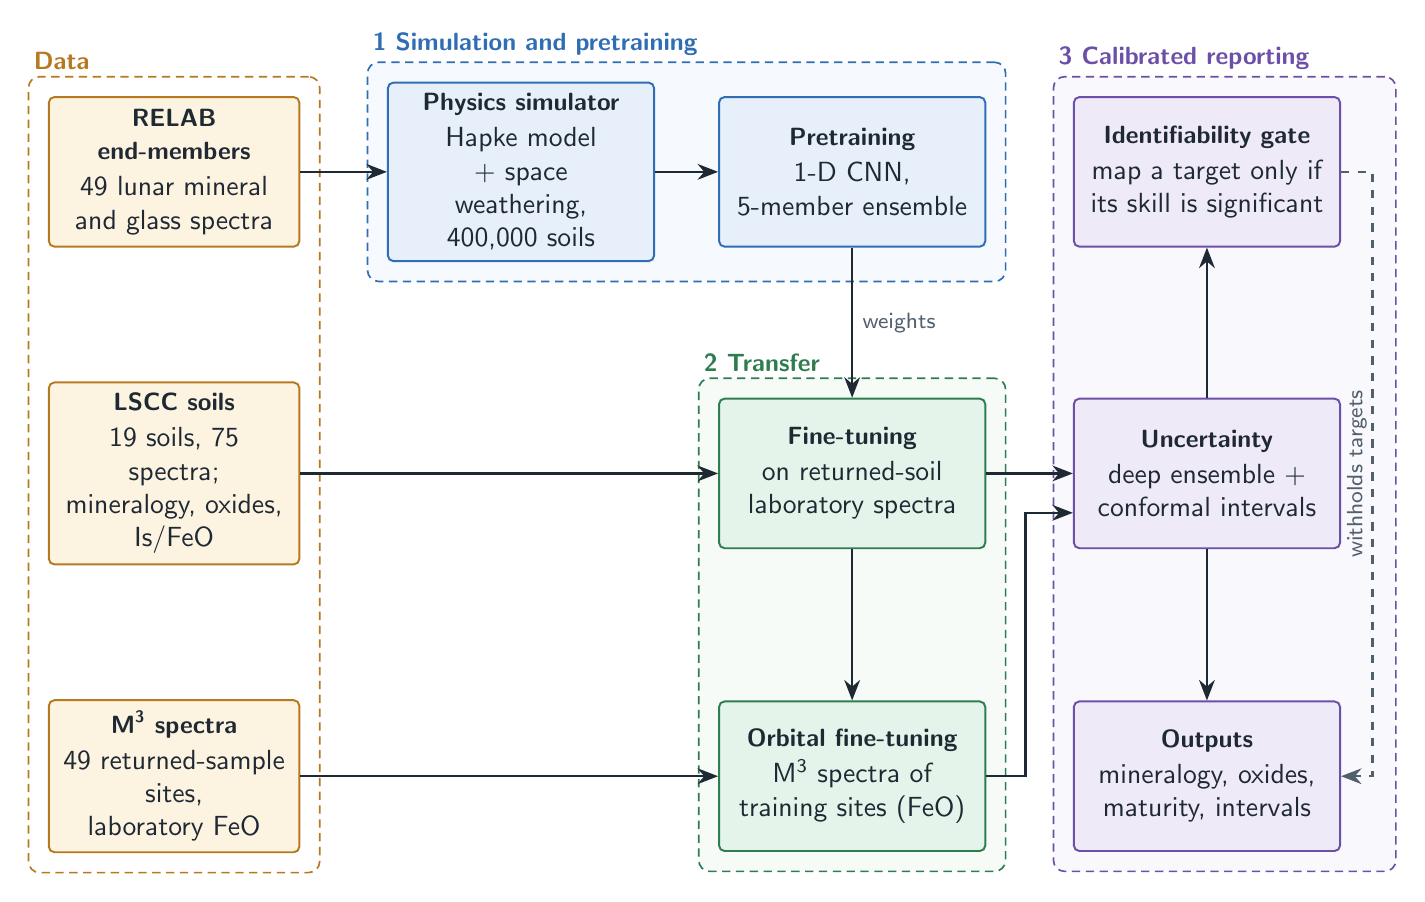
\begin{tikzpicture}[node distance=6mm and 9mm]
% ---- data column
\node[box, draw=dataS, fill=dataF, text width=29mm, minimum height=19mm] (relab) {\T{RELAB\\end-members}49 lunar mineral\\and glass spectra};
\node[box, draw=dataS, fill=dataF, text width=29mm, minimum height=19mm, below=17mm of relab] (lscc) {\T{LSCC soils}19 soils, 75 spectra;\\mineralogy, oxides,\\Is/FeO};
\node[box, draw=dataS, fill=dataF, text width=29mm, minimum height=19mm, below=17mm of lscc] (m3) {\T{M\textsuperscript{3} spectra}49 returned-sample\\sites, laboratory FeO};
% ---- stage 1
\node[box, draw=physS, fill=physF, text width=31mm, minimum height=19mm, right=11mm of relab] (sim) {\T{Physics simulator}Hapke model + space\\weathering, 400{,}000 soils};
\node[box, draw=physS, fill=physF, text width=31mm, minimum height=19mm, right=8mm of sim] (pre) {\T{Pretraining}1-D CNN,\\5-member ensemble};
% ---- stage 2
\node[box, draw=tranS, fill=tranF, text width=31mm, minimum height=19mm] (ft) at (pre |- lscc) {\T{Fine-tuning}on returned-soil\\laboratory spectra};
\node[box, draw=tranS, fill=tranF, text width=31mm, minimum height=19mm] (oft) at (pre |- m3) {\T{Orbital fine-tuning}M\textsuperscript{3} spectra of\\training sites (FeO)};
% ---- stage 3
\node[box, draw=repS, fill=repF, text width=31mm, minimum height=19mm, right=11mm of ft] (unc) {\T{Uncertainty}deep ensemble +\\conformal intervals};
\node[box, draw=repS, fill=repF, text width=31mm, minimum height=19mm] (gate) at (unc |- relab) {\T{Identifiability gate}map a target only if\\its skill is significant};
\node[box, draw=repS, fill=repF, text width=31mm, minimum height=19mm] (out) at (unc |- m3) {\T{Outputs}mineralogy, oxides,\\maturity, intervals};
% ---- arrows
\draw[arr] (relab) -- (sim);
\draw[arr] (sim) -- (pre);
\draw[arr] (pre) -- node[right, font=\footnotesize, text=muted]{weights} (ft);
\draw[arr] (lscc) -- (ft);
\draw[arr] (ft) -- (oft);
\draw[arr] (m3) -- (oft);
\draw[arr] (ft) -- (unc);
\draw[arr] (oft.east) -- ++(5mm,0) |- ($(unc.west)+(0,-5mm)$);
\draw[arr] (unc) -- (gate);
\draw[arr] (unc) -- (out);
\draw[darr] (gate.east) -- ++(4mm,0) coordinate (wh0) |- (out.east);
\node[font=\footnotesize, text=muted, rotate=90, anchor=south] (wh) at ($(wh0)!0.5!(wh0 |- out.east)+(0.5mm,0)$) {withholds targets};
% ---- stage frames
\begin{scope}[on background layer]
\node[stage, draw=dataS, fit=(relab)(m3)] (fd) {};
\node[stage, draw=physS, fill=physF!35, fit=(sim)(pre)] (f1) {};
\node[stage, draw=tranS, fill=tranF!35, fit=(ft)(oft)] (f2) {};
\node[stage, draw=repS, fill=repF!35, fit=(gate)(out)(unc)(wh)] (f3) {};
\end{scope}
\node[stagelabel, text=dataS] at (fd.north west) {Data};
\node[stagelabel, text=physS] at (f1.north west) {1\,\,Simulation and pretraining};
\node[stagelabel, text=tranS] at (f2.north west) {2\,\,Transfer};
\node[stagelabel, text=repS] at (f3.north west) {3\,\,Calibrated reporting};
\end{tikzpicture}
\end{document}
